\documentclass{beamer}

\usepackage{amsmath}
\usepackage{amssymb}
\usepackage{amsthm}
\usepackage{mathtools}
\usepackage{listings}
\usepackage{lmodern}
\usepackage{graphicx}
\usepackage{epsfig}

\graphicspath{{./images/}}

%\usetheme{Antibes}
%\usetheme{Bergen}
%\usetheme{Berlin}
%\usetheme{Boadilla}
%\usetheme{Copenhagen}
%\usetheme{Darmstadt}
\usetheme{Szeged}
%\usetheme{Warsaw}

\usecolortheme{beaver}

\definecolor{ggreen}{rgb}{0,0.6,0}
\definecolor{mygray}{rgb}{0.5,0.5,0.5}
\definecolor{mmauve}{rgb}{0.58,0,0.82}
\definecolor{backcolour}{rgb}{0.95,0.95,0.92}

\lstset{
	basicstyle=\footnotesize\ttfamily,
	numbers=left,
	stepnumber=1,
	numbersep=5pt,
	numberstyle=\small\ttfamily\color{black},
	breaklines=true,
	showstringspaces=false,
	tabsize=2,
	captionpos=b,
	commentstyle=\color{ggreen},
	escapeinside={\%*}{*)},
	keywordstyle=\color{blue},
	stringstyle=\color{mmauve},
	backgroundcolor=\color{backcolour}, 
}



\title{The Parking Problem}
\author{Jerry Kiely}
    \institute{School of Mathematical Sciences\\
	Dublin Institute of Technology\\
	Dublin 8\\
	Ireland}
\date{\today}


\begin{document}

\begin{frame}
\titlepage
\end{frame}

\begin{frame}
    \frametitle{Outline}
    \tableofcontents
\end{frame}




\section{Introduction}
\begin{frame}
    \frametitle{The Parking Problem}
    Consider an interval $(0, x)$ upon which we place a segment of unit length 
    at random. We continue by placing a second segment of unit length randomly 
    upon the original interval, discarding the segment if it overlaps with the 
    original one.
    
    We continue in this fashion until we can no longer add unit segments without 
    overlap. At each step the next position within the interval is chosen from a 
    uniform distribution of the remaining locations within the interval.
    
    We are interested in both the expected value of the number of unit segments 
    contained within the interval $(0, x)$, denoted $M(x)$, and the expected 
    filling density of unit segments within the interval, denoted $M(x) / x$.
\end{frame}

\begin{frame}
    \frametitle{Applications}
    \begin{itemize}
        \item Random Sequential Adsorption
        \item Genome Sequencing
    \end{itemize}
\end{frame}




\section{Approaches}
\begin{frame}
    \frametitle{Approaches}
    \begin{itemize}
        \item Wiener's Approach
        \item R\'enyi's Approach
        \item Kinetic Approach
        \item Generalizations Of The Kinetic Approach
    \end{itemize}
\end{frame}

\begin{frame}
    \frametitle{Wiener's Approach}
    \begin{itemize}
        \item Elementary Treatment
        \item Provides Bounds On The Limit Rather Than The Limit Itself
        \item Uses "Trial-And-Error Method"
        \item Includes An Error
        \item Unsatisfying
    \end{itemize}
\end{frame}

\begin{frame}
    \frametitle{R\'enyi's Approach}
    \begin{itemize}
        \item Analytic Treatment
        \item Computes The Limit
        \item Complicated And Convoluted
        \item Only Slightly More Satisfying
    \end{itemize}
\end{frame}

\begin{frame}
    \frametitle{R\'enyi's Approach}
	\[
		\lim_{x \to \infty} \frac{M(x)}{x} = C_R
	\]
	with
	\[
		C_R = \int_{0}^{\infty} \exp \left( -2 \int_{0}^{t} \frac{1 - e^{-u}}{u} du \right) dt
	\]
\end{frame}



\begin{frame}
    \frametitle{Kinetic Approach}
    \begin{itemize}
        \item Time Evolution Of The Distribution Of Gaps
        \item Models The Process
        \item Elegant Treatment
        \item Coverage Function Tends To The Limit
        \item Very Satisfying
    \end{itemize}
\end{frame}

\begin{frame}
	\frametitle{Kinetic Approach}
	Let $X_t$ be a random variable that represents the length of a gap at 
	time $t$, with $N(x, t)$ the number of gaps less than or equal to $x$, 
	and $N(t)$ the total number of gaps. We define the gap length 
	distribution $F(x, t)$ as follows:
	\[
		P(X_t \leq x) = F(x, t) = \frac{N(x, t)}{N(t)}
	\]
	here $P(A)$ represents the probability of event $A$ occurring.
\end{frame}

\begin{frame}
	\frametitle{Kinetic Approach}
	The gap length density function $f(x, t)$ is then:
	\[
		f(x, t) = \frac{\partial F}{\partial x} = \frac{1}{N(t)} \frac{\partial N}{\partial x} (x, t)
	\]
	therefore the probability that a gap has length between $a$ and $b$ is:
	\[
		\int_{a}^{b} f(x, t) dx = \frac{1}{N(t)} \int_{a}^{b} \frac{\partial N}{\partial x} (x, t) dx
	\]
	which is simply the number of gaps with length between $a$ and $b$ 
	divided by the total number of gaps at time $t$.
\end{frame}

\begin{frame}
	\frametitle{Kinetic Approach}
	We define the gap density function, $P(x, t)$, as:
	\[
		P(x, t) = \frac{1}{L} \frac{\partial N}{\partial x} (x, t)
	\]
\end{frame}

\begin{frame}
	\frametitle{Kinetic Approach}
	After some manipulation, the coverage function was shown to be:
	\[
		\theta(t) = \int_{0}^{\infty} P(x, t) dx
	\]
\end{frame}

\begin{frame}
	\frametitle{Kinetic Approach}
	We form a rate equation using our expressions for the gap density function: 
	\begin{eqnarray*}
		\frac{\partial P(x, t)}{\partial t} = 
		\begin{dcases}
			2 \int_{x + 1}^{\infty} P(y, t) dy                     & \text{for } x < 1 \\
			-(x - 1) P(x, t) + 2 \int_{x + 1}^{\infty} P(y, t) dy  & \text{for } x \geq 1
		\end{dcases}
	\end{eqnarray*}
	which is composed of creation and destruction terms
\end{frame}

\begin{frame}
	\frametitle{Kinetic Approach}
	The creation term may be be understood by considering a gap of length $y \geq x + 1$, 
	there are exactly two ways to park within this gap that will result in a gap of length $x$. 

	The destruction term, which only appears in the case where $x \geq 1$, deals with 
	the case where an existing gap of length $x$ is destroyed by parking a car within 
	it - in this case the remaining length becomes $x - 1$, and this destruction can be 
	accomplished in $P(x, t)$ ways.
\end{frame}

\begin{frame}
    \frametitle{Kinetic Approach}
    \[
        \lim_{\tau \to \infty} \theta(\tau) = C_R
    \]
    where
    \[
        \theta(\tau) = \int_{0}^{\tau} \exp \left( -2 \int_{0}^{t} \frac{1 - e^{-u}}{u} du \right) dt
    \]
\end{frame}

\begin{frame}
    \frametitle{Kinetic Approach}
    \begin{figure}[h!]
    	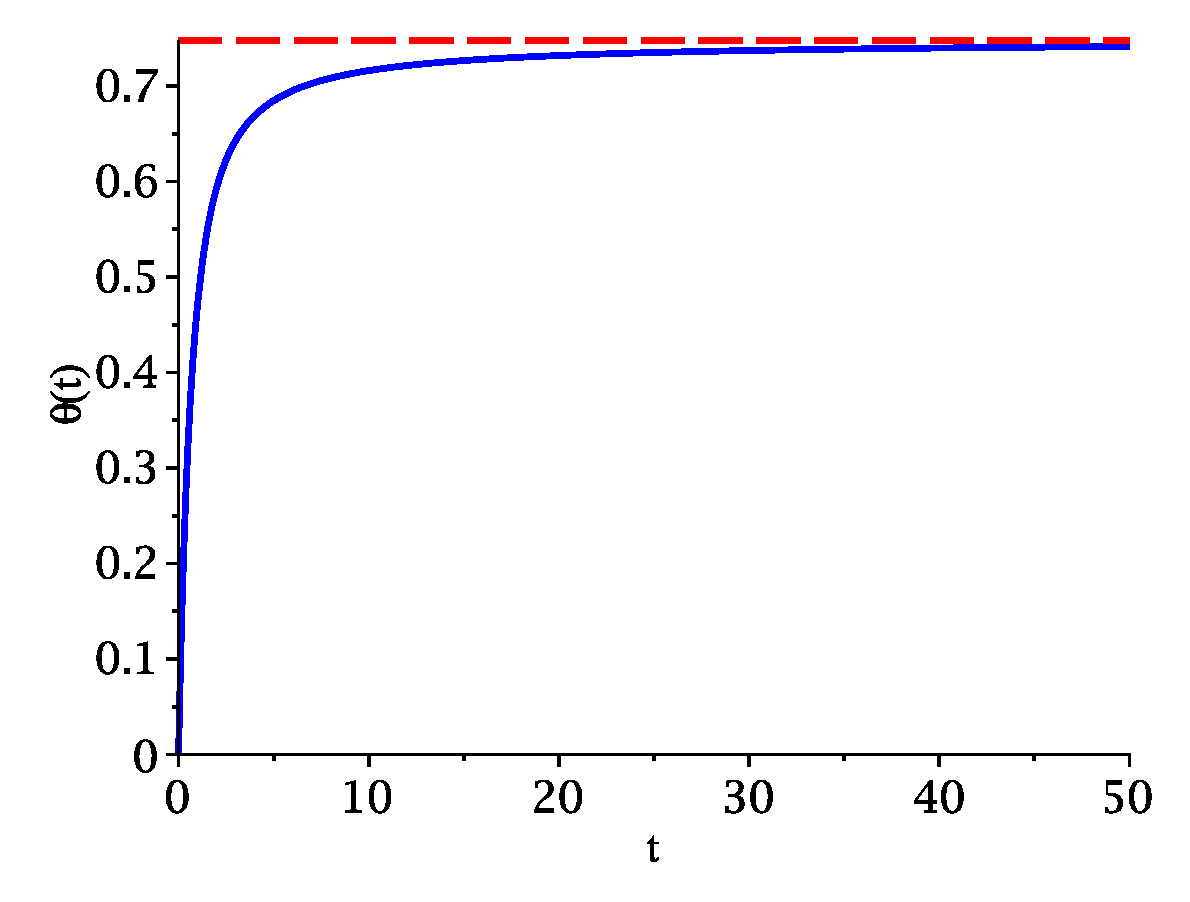
\includegraphics[scale = 0.35]{theta_01.eps}
    	\caption{The coverage function}
    \end{figure}
\end{frame}

\begin{frame}
	\frametitle{Kinetic Approach}
	It should be noted that the approach of reducing the rate equation to an ODE breaks down 
	for finite $L$.
\end{frame}

\begin{frame}
    \frametitle{Generalizations}
    \begin{itemize}
        \item Parking With Overlap
        \item Reversible Parking Problem
        \item Both Build On Kinetic Approach
        \item Again Very Satisfying
    \end{itemize}
\end{frame}

\begin{frame}[fragile]
	\frametitle{Generalizations}
	The coverage by cars for parking with overlap is:
	\begin{eqnarray*}
		\Theta_{\phi}(t) = 
		\begin{dcases}
			(1 - 2 \phi) \int_{0}^{t} F_{\phi}(\tau) d \tau  + \int_{0}^{t} F_{\phi}(\tau) \frac{2}{\tau} (1 - e^{-\phi \tau}) d \tau			& \text{for } \phi < \frac{1}{2} \\
			1 - F_{\phi}(t) e^{(1 - 2 \phi)t}																									& \text{for } \phi \geq \frac{1}{2} 
		\end{dcases}
	\end{eqnarray*}
\end{frame}

\begin{frame}[fragile]
	\frametitle{Generalizations}
	The the equilibrium coverage for the reversible parking problem is:
	\begin{eqnarray*}
			\theta_{eq} & =       & \frac{\alpha}{1 + \alpha} \\
						& \approx & 1 - \frac{1}{\ln(k_{+}/k_{-})} 
	\end{eqnarray*}
\end{frame}








\section{Simulations}
\begin{frame}
    \frametitle{Monte Carlo Approach}
	\begin{itemize}
		\item define the range of values to be drawn from
		\item draw values from this range using a distribution
		\item perform a computation on the results 
		\item record the results of the computation
		\item repeat as appropriate
	\end{itemize}
\end{frame}

\begin{frame}
	\frametitle{Monte Carlo Approach}
	A Method 
	\begin{itemize}
		\item For Evaluating Results
		\item For Confirming Theories
		\item Best Applied To Problems With A Probabilistic Element
	\end{itemize}
\end{frame}

\begin{frame}[fragile]
    \frametitle{The Parking Problem Simulation - Discrete Version}
    \begin{itemize}
        \item a length $L$ made up of discrete sites 
        \item attempt to park cars that occupy two adjacent sites
        \item the process is successful if a car tries to park at two adjacent empty sites
        \item otherwise unsuccessful
        \item the process continues until there are no more free adjacent empty sites 
    \end{itemize}
\end{frame}

\begin{frame}[fragile]
    \frametitle{The Parking Problem Simulation - Discrete Version}
    The coverage for the discrete parking problem is $\theta_{d}(t)$, and the jamming coverage is: 
    \[
    	\lim_{t \to \infty} \theta_{d}(t) = 1 - e^{-2}
    \]
    which is calculated to be $0.864664$ to six decimal places.
\end{frame}

\begin{frame}[fragile]
    \frametitle{The Parking Problem Simulation - Discrete Version}
	\begin{lstlisting}[numbers=none]
    Parking Problem - Discrete Version: results

                                     L:   100000
                            iterations:    10000

                          distribution:
                                  mean: 0.864673
                    standard deviation: 0.000848

	\end{lstlisting}
\end{frame}

\begin{frame}
    \begin{figure}
    	\centering
    	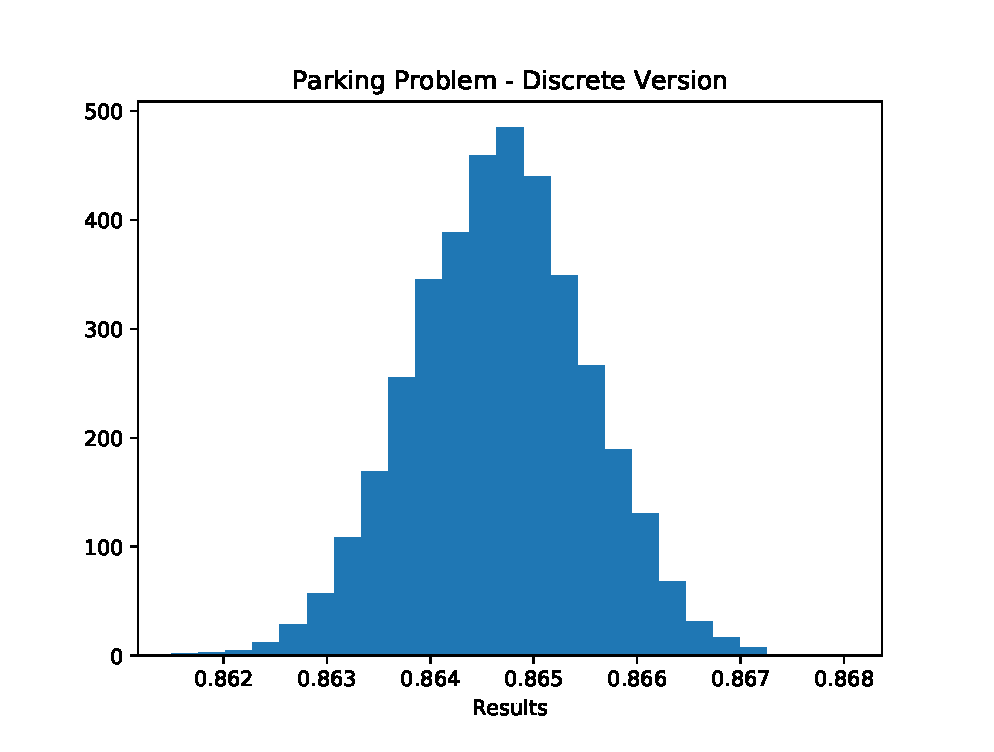
\includegraphics[scale = 0.5]{parking_simulation_01.eps}
    	\caption{Histogram of the parking problem simulation - discrete case}
    \end{figure}
\end{frame}

\begin{frame}[fragile]
	\frametitle{The Parking Problem Simulation - Discrete Version}
	The results of the simulation for the discrete parking problem are consistent with the 
	theory. 
\end{frame}

\begin{frame}[fragile]
    \frametitle{The Parking Problem Simulation}
	\begin{lstlisting}[numbers=none]
                    Parking Problem: results

                                  L:   100000
                         iterations:    10000

                       distribution:
                               mean: 0.747602
                 standard deviation: 0.000617

	\end{lstlisting}
\end{frame}

\begin{frame}
    \begin{figure}
    	\centering
    	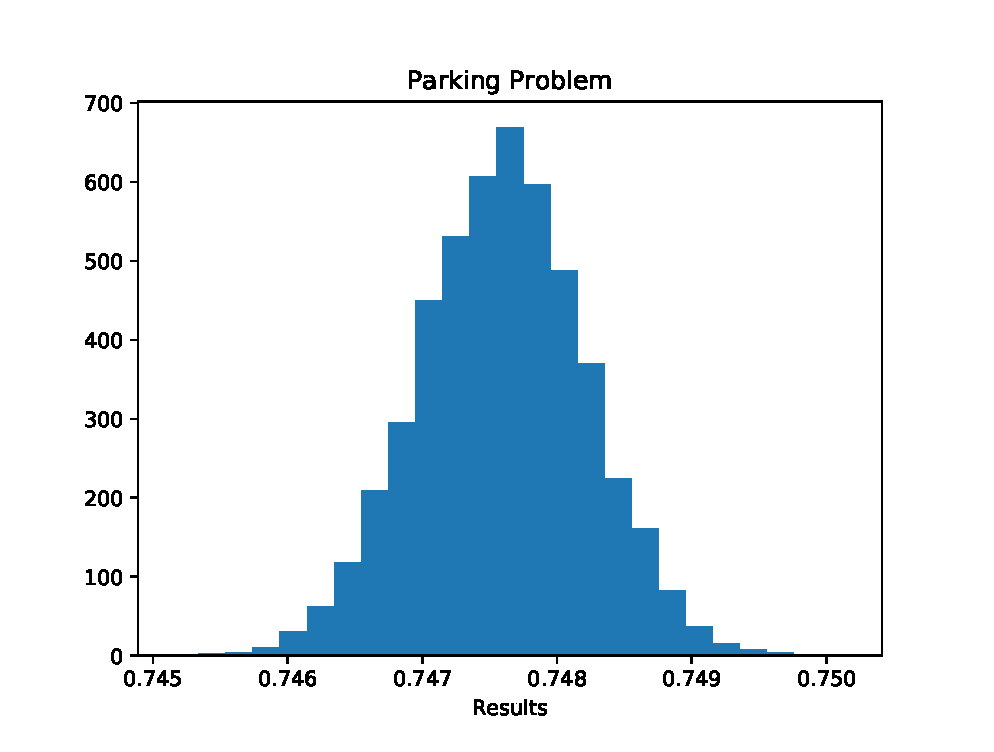
\includegraphics[scale = 0.5]{parking_simulation_02.eps}
    	\caption{Histogram of the parking problem simulation}
    \end{figure}
\end{frame}

\begin{frame}[fragile]
    \frametitle{The Parking Problem Simulation - Overlap Version}
    The coverage by cars for parking with overlap is:
    \begin{eqnarray*}
    	\Theta_{\phi}(t) = 
    	\begin{dcases}
    		(1 - 2 \phi) \int_{0}^{t} F_{\phi}(\tau) d \tau  + \int_{0}^{t} F_{\phi}(\tau) \frac{2}{\tau} (1 - e^{-\phi \tau}) d \tau			& \text{for } \phi < \frac{1}{2} \\
    		1 - F_{\phi}(t) e^{(1 - 2 \phi)t}																									& \text{for } \phi \geq \frac{1}{2} 
    	\end{dcases}
    \end{eqnarray*}
\end{frame}

\begin{frame}
    The jamming coverage for a selection of values of $\phi$ 
    as $t \to \infty$ is shown below:
    \begin{table}
    	\centering
    	\begin{tabular}{|l | l|} 
    		\hline
    		$\phi$ & $\lim_{t \to \infty} \Theta_{\phi}(t)$ \\ [1ex] 
    		\hline
    		0.1 & 0.816909 \\ 
    		0.2 & 0.880028 \\ 
    		0.3 & 0.936238 \\ 
    		0.4 & 0.980342 \\ 
    		0.5 & 1 \\ 
    		\hline
    	\end{tabular}
    	\caption{$\lim_{t \to \infty} \Theta_{\phi}(t)$}
    	\label{table:2}
    \end{table}
    The coverage gets closer to full coverage (i.e. $1$) as $\phi \to 0.5$. \bigskip
\end{frame}

\begin{frame}[fragile]
    \frametitle{The Parking Problem Simulation - Overlap Version}
	\begin{lstlisting}[numbers=none]
    Parking Problem - Overlap Version: results

                                    L:   100000
                              overlap:      0.1
                           iterations:    10000

                         distribution:
                                 mean: 0.816894
                   standard deviation: 0.000584

	\end{lstlisting}
\end{frame}

\begin{frame}
    \begin{figure}
    	\centering
    	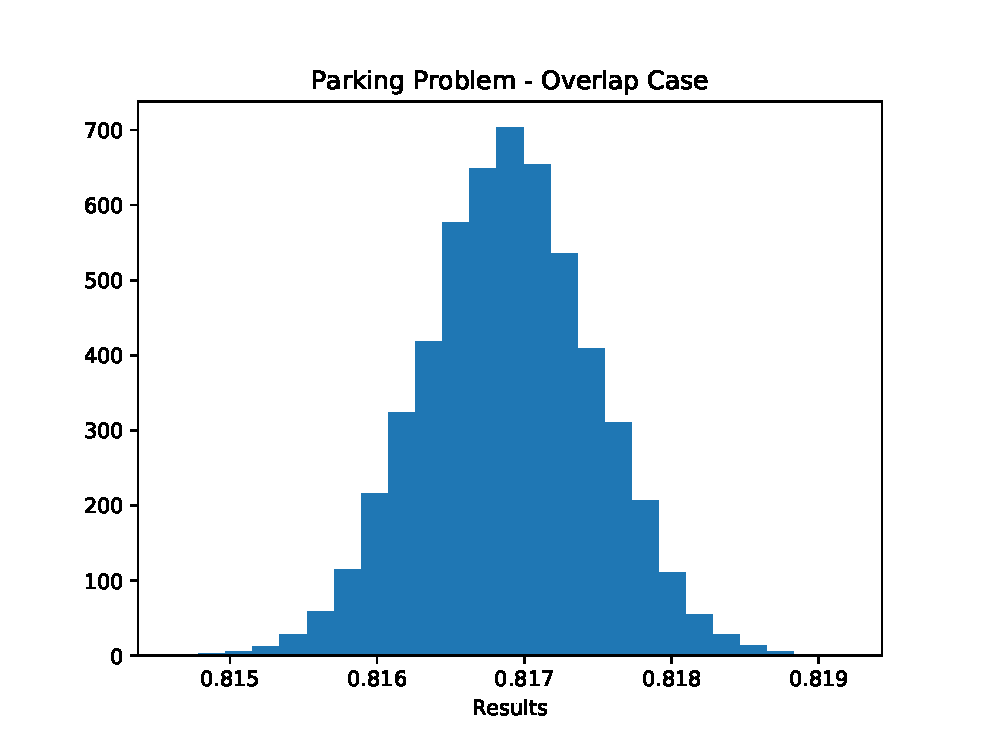
\includegraphics[scale = 0.5]{parking_simulation_03.eps}
    	\caption{Histogram of the parking with overlap simulation - $\phi = 0.1$}
    \end{figure}
\end{frame}

\begin{frame}[fragile]
	\frametitle{The Parking Problem Simulation - Overlap Version}
	\begin{lstlisting}[numbers=none]
    Parking Problem - Overlap Version: results

                                    L:   100000
                              overlap:      0.2
                           iterations:    10000

                         distribution:
                                 mean: 0.880027
                   standard deviation: 0.000477
	
	\end{lstlisting}
\end{frame}

\begin{frame}
	\begin{figure}
		\centering
		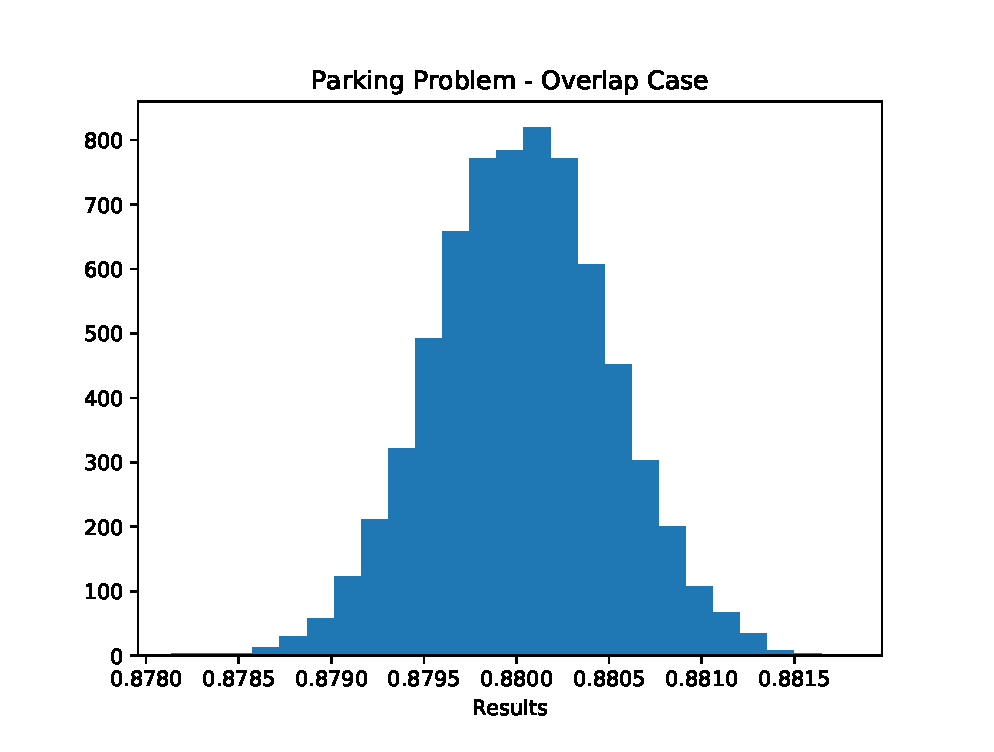
\includegraphics[scale = 0.5]{parking_simulation_04.eps}
		\caption{Histogram of the parking with overlap simulation - $\phi = 0.2$}
	\end{figure}
\end{frame}

\begin{frame}[fragile]
	\frametitle{The Parking Problem Simulation - Overlap Version}
	\begin{lstlisting}[numbers=none]
    Parking Problem - Overlap Version: results

                                    L:   100000
                              overlap:      0.3
                           iterations:    10000

                         distribution:
                                 mean: 0.936235
                   standard deviation: 0.000327
	
	\end{lstlisting}
\end{frame}

\begin{frame}
	\begin{figure}
		\centering
		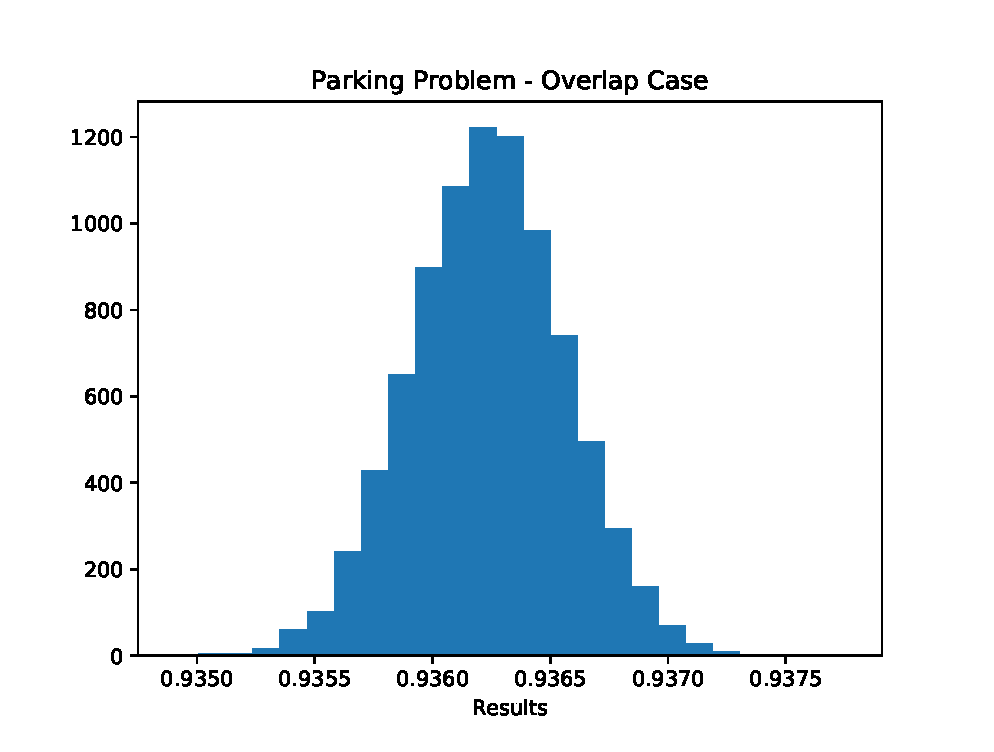
\includegraphics[scale = 0.5]{parking_simulation_05.eps}
		\caption{Histogram of the parking with overlap simulation - $\phi = 0.3$}
	\end{figure}
\end{frame}

\begin{frame}[fragile]
	\frametitle{The Parking Problem Simulation - Overlap Version}
	\begin{lstlisting}[numbers=none]
    Parking Problem - Overlap Version: results

                                    L:   100000
                              overlap:      0.4
                           iterations:    10000

                         distribution:
                                 mean: 0.980344
                   standard deviation: 0.000144

	\end{lstlisting}
\end{frame}

\begin{frame}
	\begin{figure}
		\centering
		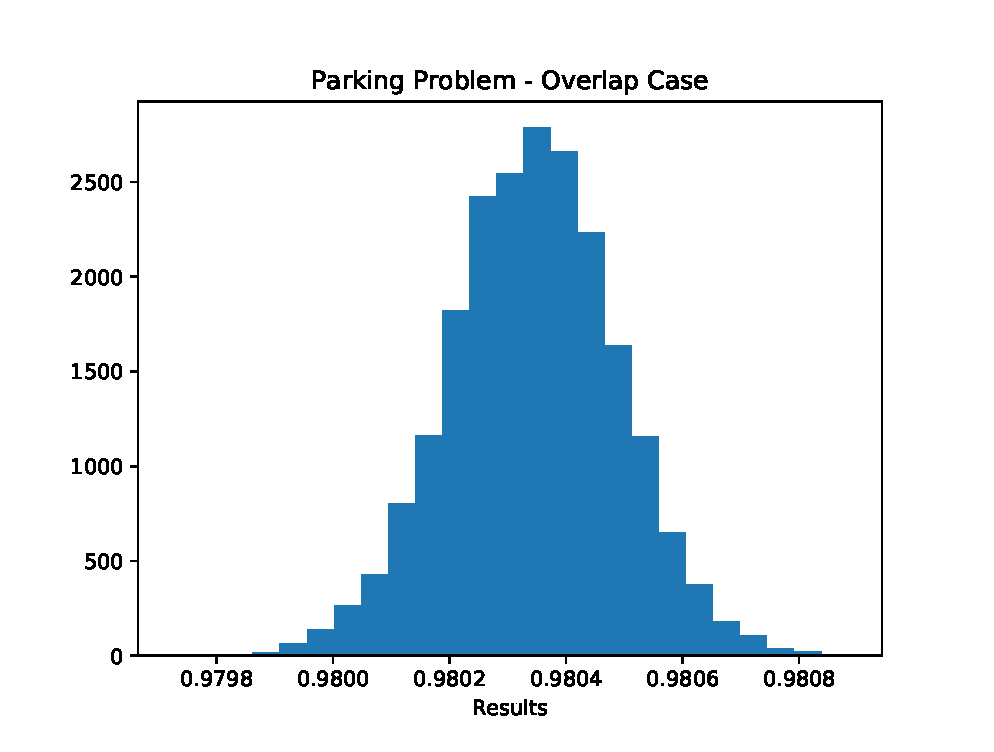
\includegraphics[scale = 0.5]{parking_simulation_06.eps}
		\caption{Histogram of the parking with overlap simulation - $\phi = 0.4$}
	\end{figure}
\end{frame}

\begin{frame}[fragile]
    \frametitle{The Parking Problem Simulation - Overlap Version}
	\begin{lstlisting}[numbers=none]
    Parking Problem - Overlap Version: results

                                    L:   100000
                              overlap:      0.5
                           iterations:    10000

                         distribution:
                                 mean: 1.000000
                   standard deviation: 0.000000

	\end{lstlisting}
\end{frame}

\begin{frame}
    \begin{figure}
    	\centering
    	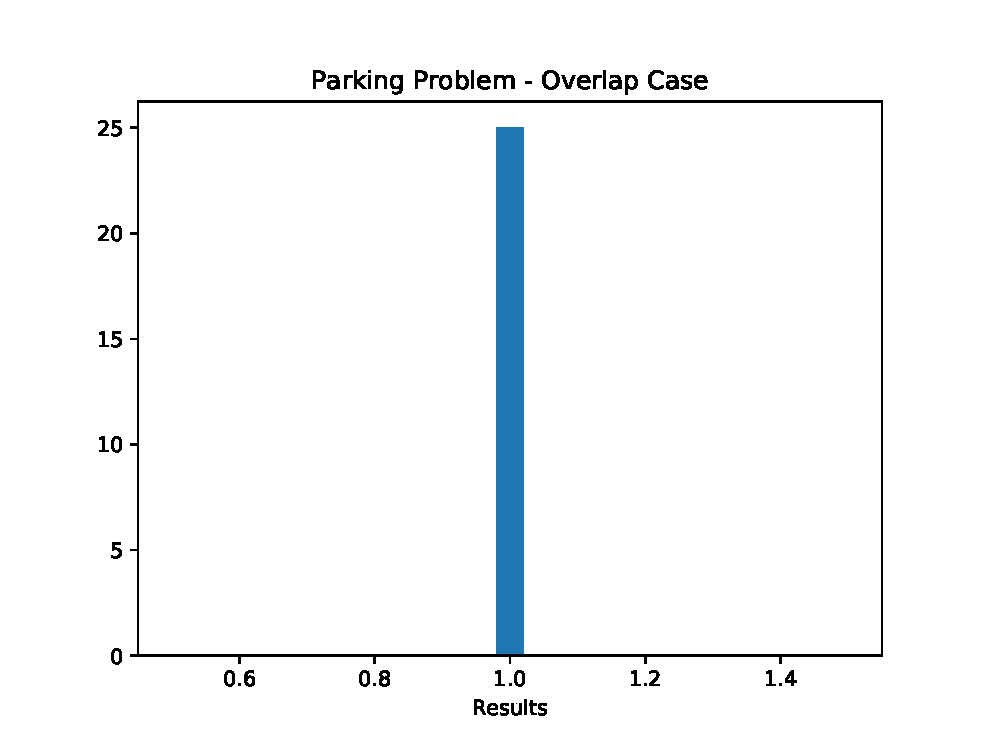
\includegraphics[scale = 0.5]{parking_simulation_07.eps}
    	\caption{Histogram of the parking with overlap simulation - $\phi = 0.5$}
    \end{figure}
\end{frame}

\begin{frame}
    \frametitle{Simulations - Trade-offs}
	\begin{itemize}
		\item high accuracy of outcome - lots of iterations, set $L$ to be as large as possible
		\item confirmation of theory - fewer iterations, shorter $L$ will suffice
		\item calculation of a value - recursive approach
	\end{itemize}\medskip
\end{frame}




\section{Conclusions}
\begin{frame}
	\frametitle{Remarks}
	Is there some underlying conservation law other than the obvious:
	\[
		\int_{0}^{\infty} x P(x, t) dx + \int_{0}^{\infty} P(x, t) dx = 1
	\]
	i.e that the normalized sum of the car lengths and gap lengths equals 1. 
\end{frame}

\begin{frame}
	\frametitle{Remarks}
	Specifically the reversible problem, and it's condition for equilibrium:
	\[
		\frac{\partial P(x, t)}{\partial t} = 0
	\]
	might lead one to believe that there are underlying conservation laws and 
	hidden symmetries at play.
\end{frame}

\begin{frame}
	\frametitle{Remarks}
	When it comes to modelling a problem that does not lend itself easily to 
	empirical verification, such as the parking problem, a simulation can tell 
	you if your theory makes sense very quickly.
\end{frame}

\begin{frame}
	\frametitle{Remarks}
	A simulation can help provide statistical properties relating to the 
	associated constants of a process, which in turn can help establish 
	whether a process is being inhibited by some unknown factor.
\end{frame}

\begin{frame}
	\frametitle{Future Research}
	$C_R$ feels like something universal, akin to $e$ or $\phi$. In 
	particular $\pi$.
\end{frame}

\begin{frame}
	\frametitle{Future Research}
	Higher dimensional problems, in two and three dimensions. Investigating 
	what (if any) relationship exists between two and three dimensional 
	packing problems and $C_R$.
\end{frame}

\begin{frame}
	\frametitle{Future Research}
	Competitive RSA of a binary mixture - where cars of two different lengths 
	compete for parking spaces. A more complicated problem mathematically, and 
	more difficult to simulate.
\end{frame}

\begin{frame}
	\frametitle{Finally}
	Thank you for your time and patience.
\end{frame}




\end{document}

